\documentclass{article}
\usepackage[utf8]{inputenc}
\usepackage[margin=25mm]{geometry}
\usepackage{float}
\usepackage[english]{babel}
\usepackage{authblk}
\usepackage{natbib}
\usepackage[export]{adjustbox}% http://ctan.org/pkg/adjustbox
\usepackage{subfiles}
\usepackage{mathtools}
\usepackage{xurl}
\usepackage{pdflscape}
\usepackage{graphicx}
\usepackage{tikz}
\usepackage{lineno}
\usepackage{adjustbox}
\usepackage{setspace}
\usepackage{dsfont}

\newcommand{\beginsupplement}{
        \setcounter{table}{0}
        \renewcommand{\thetable}{S\arabic{table}}%
        \setcounter{figure}{0}
        \renewcommand{\thefigure}{S\arabic{figure}}%
}



\begin{document}
\title{A simple test to uncover signals of CpG hypermutability using posterior predictive simulations}
\author[1]{Simon Laurin-Lemay}
\author[1,2,3]{Nicolas Rodrigue}
\affil[1]{Department of Biology, Carleton University, Ottawa, Canada}
\affil[2]{Institute of Biochemistry, Carleton University, Ottawa, Canada}
\affil[3]{School of Mathematics and Statistics, Carleton University, Ottawa, Canada}
\date{}
\maketitle
\section*{Keywords}
DNA sequence evolution, Markov chain Monte Carlo, phylogenetics, misspecification, confounding factors
\section*{Declarations}
Conflict of interest: The authors declare that they have no competing
interests.
\section*{Correspondence}
Simon Laurin-Lemay\\
209 Nesbitt Biology Building,\\
1125 Colonel By Drive Ottawa,\\
Ontario, CANADA\\
K1A 0C6\\
evol.simon@gmail.com\\
% tel: +1 613 520 2600 x 41941\\
\clearpage
\doublespacing

\section*{Abstract}
CpG hypermutability is caused by the spontaneous deamination of methylated cytosines within CpG contexts and is known to impact vertebrate evolution.  The phenomenon has been shown to confound tests of selection in protein-coding genes.  In this work, we propose a simple test based on the use of posterior predictive sampling to detect the presence of CpG hypermutability using common nucleotide substitution models.  Artificial data sets were generated using a jump-chain simulation algorithm with a model incorporating varying levels of CpG hypermutability.  On simulations using realistic parameter values, we recovered between 0-8\% of false positives and no false negatives.  We then ran the test on 137 mammalian gene alignments, all of which were found to exhibit CpG hypermutability, corroborating previous studies based on elaborate and computationally expensive Monte Carlo methods.  For greater confidence in its results, any study aimed at detecting signals of selection could easily be accompanied by this simple test.

\clearpage
\linenumbers
\section*{Introduction}
All models, by definition, make simplifying assumptions about the phenomena they attempt to capture.  One of the risks associated with these simplifications is that true features that are unaccounted for could mislead the model-based inferences being conducted.  For example, the hypermutability of CpGs due to the process of spontaneous deamination of methylated cytosines in CpG contexts \citep{Bird1980,Burge1992} can confound model-based detection of selection, potentially leading to erroneous conclusions regarding codon usage preferences \citep{LaurinLemay2018a}, or positive selection at the amino acid level \citep{LaurinLemay2022}.

Most substitution models assume that sites evolve independently, which is particularly convenient for calculating the phylogenetic likelihood function; one only need multiply all the site likelihoods, calculated independently from each site of the alignment \citep{Felsenstein1981}.  On the other hand, implementing substitution processes taking into account dependencies between sites \citep[e.g.,][]{Robinson2003,Rodrigue2009,LaurinLemay2018b,Meyer2019}, as required to parameterize the hypermutability of CpGs, is not a trivial task.  Some of the strategies employed have included nested Markov chain Monte Carlo sampling \citep[e.g.,][]{Robinson2003,Rodrigue2009} and simulation-based Approximate Bayesian Computation \citep[e.g.,][]{LaurinLemay2018b}.  In all cases, the methods are computationally elaborate and costly.

Short of explicitly modeling site-dependencies, simulation-based methods, such as parametric bootstrapping \citep{Efron1979,Efron1993} or posterior predictive sampling \citep{Gelman1996,Brown2018}, can be utilized to uncover site-dependent features having the potential to mislead inferences.  Here, we propose a simple posterior predictive test based on the widely used GTR+$\Gamma$ model to uncover a statistical signal of CpG hypermutability in mammalian genes.  In the presence of CpG hypermutability, we expect the GTR+$\Gamma$ substitution model to predict more CpG dinucleotides than would be observed in real alignments, because CpG hypermutability is not accounted for in the model definition, and hence CpG dinucleotides do not become depleted when simulating the evolutionary process over the phylogeny.

\section*{CpG hypermutability test}
The CpG test consists of calculating the proportion of times, i.e., \emph{p-value}, that the frequency of CpGs calculated from the real alignment is greater than the CpG frequency recovered from the posterior predictive alignments, which are generated by simulation over a sample of parameter values drawn from their posterior distribution by Markov chain Monte Carlo under the GTR+$\Gamma$ model.  The following equation details the CpG test:

\begin{equation}\label{test}
 \text{\emph{p-value}} = \frac{1}{N}\sum_{i=1}^{N}\delta(freq_{CpG}^{real}>freq_{CpG}^{pred_{i}}),
\end{equation}
where $N$ is the predictive sample size, $freq_{CpG}^{real}$ refers to the frequency of CpG dinucleotides in the real alignment, $freq_{CpG}^{pred_{i}}$ is the CpG dinucleotide frequency of the $i$th posterior predictive alignment, and $\delta$ is an indicator function that returns 1 if the CpG frequency calculated from the real alignment is greater than the predictive CpG frequency and 0 otherwise.  With this simple test-statistic, a \emph{p-value} close to 0 suggests a rejection of a null hypothesis of absence of a CpG hypermutability process governing the real data relative to the simulations.  Crudely, a threshold (\emph{p-value} $<0.05$) can be chosen to flag a data set as a \emph{positive} for potential CpG hypermutability, and \emph{negative} otherwise.

\section*{Simulation study}
We analyzed 10 mammalian protein-coding gene alignments selected for their wide range of GC content \citep{LaurinLemay2018b}.  We used these alignments to obtain parameter values for simulations under the GTR+$\Gamma$ substitution model, providing the simplest \emph{negative controls}: synthetic data sets that have no signal of CpG hypermutability.  For each gene, we used ten draws from the posterior distribution, approximated using PhyloBayes-MPI \citep{Lartillot2013}, as parameters for simulations under GTR+$\Gamma$, conducted with AliSim \citep{LyTrong2022}, thereby yielding 100 simulated alignments in total.

We next conducted simulations for \emph{positive controls}: synthetic data sets produced under an evolutionary process that includes CpG hypermutability.  In this case, we used the MG-F1$\times$4 codon substitution model \citep[see, e.g.,][for a detailed description]{Rodrigue2008} within Phylobayes-MPI \citep{Rodrigue2014}.  The latter provided parameter values for nucleotide frequencies and pairwise exchangeabilities, but for two key parameters of our codon-level simulations, we explored two different values each: the nonsynonymous/synonymous rate ratio, $\omega$, was set to either 0.2 or 1, and a parameter controlling CpG hypermutability, $\lambda$ \citep[see][for a detailed description]{LaurinLemay2018b}, was set to either 4 or 8, reflecting empirical values commonly observed on real data \citep{LaurinLemay2018b}.  Note that another negative control can be obtained by setting $\lambda=1$, which we also investigated.  From the 10 sets of parameter values drawn for the posterior distribution under MG-F1$\times$4 for each of the 10 alignments, with all combinations of $\omega$ and $\lambda$ values, we thus simulated 600 synthetic alignments.

Each negative control and positive control alignment was then analyzed with the CpG hypermutability test.  Less than 5\% of the tests were significant when performed on synthetic sequence alignments generated under the GTR+$\Gamma$ substitution model, i.e., 2\% (Table \ref{tab:table_1}).  Similarly, none of the CpG tests were significant when performed on synthetic sequence alignments generated without CpG hypermutability and with $\omega = 0.2$ using the MG-F1$\times$4 codon substitution model, and 8\% were significant with $\omega=1$ (Table \ref{tab:table_1}).  On the other hand, in the presence of CpG hypermutability all tests were positive.

\subsection*{Empirical study}
We retrieved the 137 mammalian codon alignments from \citet{LaurinLemay2018a} along with the tree topology.  We applied the posterior predictive CpG hypermutability test to each of them and found 100\% of the tested genes to be significant (\emph{p-value}$=0$, $\alpha=0.05$).  In other words, CpG frequencies are significantly reduced in all real alignments compared to frequencies recovered from predicted alignments generated by the GTR$+\Gamma$ substitution model.  As an example, in Figure \ref{fig:figure_1}, panel A, we show the discrepancy between the CpG frequencies predicted by GTR$+\Gamma$ and the observed CpG frequency in one of the examined coding sequence alignments.  On the same alignment, panel B shows that the true value of the frequency of another dinucleotide, ApT, falls within the posterior predictive distribution.  The test thus suggests that something is unaccounted for with regards to CpG frequencies in particular.

\section*{Discussion}
The approach proposed herein is crude, with uncalibrated posterior predictive \emph{p-values}.  However, it is quick and easy to implement, and clearly highlights the presences of CpG hypermutability.  Knowing that CpG hypermutability can mislead tests for selection \citep{LaurinLemay2018a,LaurinLemay2022}, this simple test could be systematically applied when conducting selection analyses \citep[e.g.,][]{Kosiol2008,Murrell2015,Davydov2019,Slodkowicz2020}, at relatively low cost.

More generally, however, we propose that numerous simple test-statistics could be employed within posterior predictive (or parametric bootstrap) analyses.  These include all possible dinucleotides, trinucleotides, codon boundary contexts, adjacent amino acids, average effective number of amino acids (or nucleotides, or codons) across positions, compositional heterogeneity measures of several types, and many more.  This could help contextualize the interpretation of evolutionary studies, either giving greater confidence in their results, or emphasizing where one should be cautious due to glaring model violations.

Such tests would provide a technically simple means of guiding modeling efforts.  Historically, model developers have chosen to focus on one or another hypothesized aspect of the evolutionary process to build within an existing modeling framework, without much of a systematic outline of the most prevalent or most pronounced model violations.  In many cases, newly proposed models have been years in the making, requiring the invention or recombination of novel Monte Carlo approaches, the development of new and complex computing software, self-validation simulation checks, testing, and so forth.  To date, it is quite unclear if these modeling efforts have been undertaken in rational manner, in terms of order of priority.

Our simple and crude test of CpG hypermutability is an example of how, with the tools and models we have had for decades, we can bring forth complex features of the evolutionary process from any multiple sequence alignment.  This calls for a much broader simulation-based outline of modeling objectives, both to retrospectively evaluate the sequence of modeling achievements to date, and plan more carefully for future work.

\section*{Availability of data and materials}
Workflow and data are available on the GitHub repository \url{https://github.com/Simonll/CpG-ppred-test.git}.

\section*{Acknowledgments}
This work was funded by the Natural Sciences and Engineering Research Council of Canada.

\section*{Contributions}
Conceptualization: SLL, NR. Formal analysis: SLL Investigation: SLL, NR. Methodology: SLL, NR. Resources: SLL, NR. Supervision: NR Writing original draft: SLL, NR. Review and editing: SLL, NR. \\
All authors read and approved the final manuscript.

\section*{Competing interests}
The authors declare that they have no competing interests.

\newpage
\section*{Figures}

\begin{figure}[H]
  \centering
  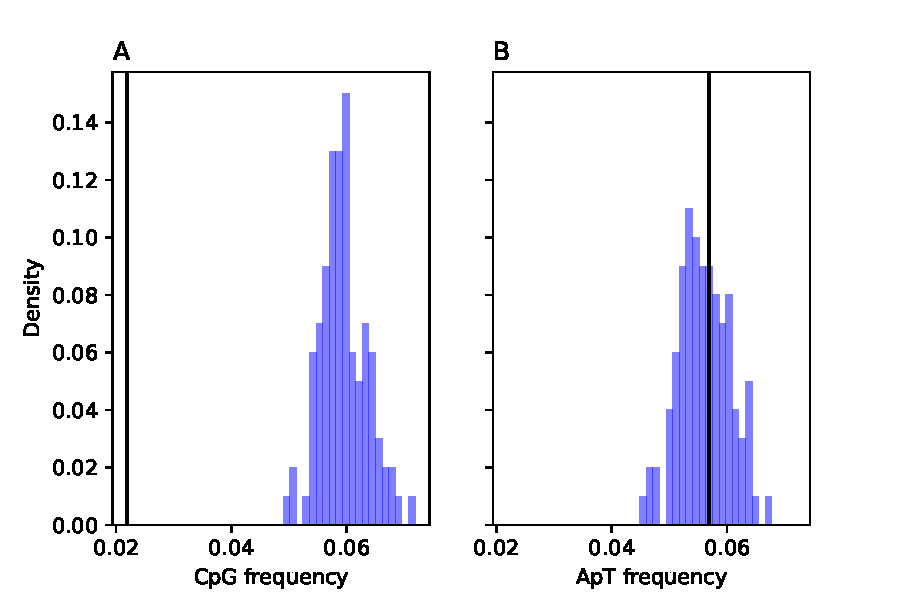
\includegraphics[width=\textwidth,height=\textheight,keepaspectratio]{figures/figure1.pdf}
  \caption{Comparison of CpG (A) and ApT (B) frequencies computed from the \emph{MEP1A} mammalian protein-coding gene alignment, black vertical lines, and corresponding frequencies computed from posterior predictive alignments generated using the GTR+$\Gamma$ substitution model, blue histograms. Note that the predicted CpG frequencies (A) overestimate the true value 100\% of the time, while the true ApT frequency (B) falls within the distribution of predicted frequencies.}
  \label{fig:figure_1}
\end{figure}

\newpage
%\begin{landscape}
\section*{Tables}

\begin{table*}[h]
    \begin{tabular}{cccccc}
    type of controls & models used to generate the synthetic alignments & positive tests (\%)\\
    \hline
    negative & GTR+$\Gamma$                              & 2\\
    negative & MG-F1$\times$4+($\lambda=1$)+($\omega=0.2$) & 0\\
    negative & MG-F1$\times$4+($\lambda=1$)+($\omega=1.0$) & 8\\
    positive & MG-F1$\times$4+($\lambda=4$)+($\omega=0.2$) & 100\\
    positive & MG-F1$\times$4+($\lambda=4$)+($\omega=1.0$) & 100\\
    positive & MG-F1$\times$4+($\lambda=8$)+($\omega=0.2$) & 100\\
    positive & MG-F1$\times$4+($\lambda=8$)+($\omega=1.0$) & 100\\
    \hline
    \end{tabular}
    \caption{Validation of the CpG test using posterior predictive sampling under the GTR+$\Gamma$ substitution model with a $\alpha$ significance threshold of 5\%. Synthetic alignments were generated using GTR+$\Gamma$ and MG-F1$\times$4 codon substitution model using three CpG hypermutability values, $\lambda = \{1,4,8\}$ and global selection on amino acids using two $\omega$ values (i.e., 0.2 and 1).}\label{tab:table_1}
\end{table*}
%\end{landscape}
\newpage
\bibliographystyle{spbasic}
\bibliography{refs}

\end{document}
